\section{Auswertung}
\label{sec:Auswertung}

Nun sollen die Brechungsindizes $n$ bestimmt werden.
Diese werden bei paralleler und senkrechter Polarisation benötigt.
Die beiden Gleichungen werden aus \autoref{eq:tbd} und \autoref{eq:tbd} extrahiert.
Als Referenzstrom wird $I_r = 167 \unit{\nano\meter}$ gemessen.


\subsection{Der Brechungsindex bei Polarisation senkrechter Ausrichtung}

Allgemein gilt die Proportionalität 
\begin{equation}
  \frac{I_r}{I_e} \thicksim \frac{E_r^2}{E_e} = E^2.
\end{equation}
Durch diese Beziehung lässt sich \autoref{eq:tbd} zu der Form
\begin{equation*}
  E_{\perp}=\left|\frac{\left(\cos ^{2}(\alpha) - \sqrt{n^{2}-\sin ^{2}(\alpha)} \right)^{2}}{n^{2}-1}\right|
\end{equation*}
umstellen.
Diese lässt sich nach $n$ umformen.
Das ergibt
\begin{equation}\label{eq:n1}
  \sqrt{1 + \frac{4 E \cos ^2(\alpha)}{(E - 1)^2}}.
\end{equation}
In \autoref{tab:mess1} sind die Messwerte und das jeweilige errechnete $n$ aufgetragen.

Wird $n$ gemittelt ergibt sich ein Brechungsindex von 
\begin{equation*}
  n_{\perp} = 4.8 ± 8.9. 
\end{equation*}


\begin{table}
  \centering
  \caption{Die Messwerte und die Ergebnisse der Rechnung.}
  \label{tab:mess1}
  \begin{tabular}{c c c c c c c c}
    \toprule
    $\alpha / °$ &     $I / \unit{\milli\ampere}$ & $\frac{I_\text{gem}}{I_\text{ref}}$ & n &$\alpha / °$ &    $I / \unit{\milli\ampere}$ & $\frac{I_\text{gem}}{I_\text{ref}}$& n \\
    \midrule
       6,0 & 0,013 &  0,092857 & 1,167118 &48 & 0,086 & 0,614286 &  2,218190 \\
       8,0 & 0,015 &  0,107143 & 1,193855 &50 & 0,088 & 0,628571 &  2,211720 \\
      10,0 & 0,015 &  0,107143 & 1,191895 &52 & 0,093 & 0,664286 &  2,302198 \\
      12,0 & 0,020 &  0,142857 & 1,261561 &54 & 0,096 & 0,685714 &  2,322735 \\
      14,0 & 0,021 &  0,150000 & 1,272628 &56 & 0,100 & 0,714286 &  2,377642 \\
      16,0 & 0,025 &  0,178571 & 1,328640 &58 & 0,106 & 0,757143 &  2,518670 \\
      18,0 & 0,027 &  0,192857 & 1,353637 &60 & 0,106 & 0,757143 &  2,399442 \\
      20,0 & 0,030 &  0,214286 & 1,393850 &62 & 0,113 & 0,807143 &  2,589478 \\
      22,0 & 0,033 &  0,235714 & 1,433663 &64 & 0,116 & 0,828571 &  2,593267 \\
      24,0 & 0,038 &  0,271429 & 1,507659 &66 & 0,120 & 0,857143 &  2,646371 \\
      26,0 & 0,040 &  0,285714 & 1,529146 &68 & 0,126 & 0,900000 &  2,833082 \\
      28,0 & 0,047 &  0,335714 & 1,643088 &70 & 0,130 & 0,928571 &  2,901770 \\
      30,0 & 0,050 &  0,357143 & 1,682241 &72 & 0,130 & 0,928571 &  2,656563 \\
      32,0 & 0,058 &  0,414286 & 1,829007 &74 & 0,140 & 1,000000 &  3,278201 \\
      34,0 & 0,060 &  0,428571 & 1,845555 &76 & 0,142 & 1,014286 &  3,143644 \\
      36,0 & 0,066 &  0,471429 & 1,956716 &78 & 0,146 & 1,042857 &  3,249584 \\
      38,0 & 0,068 &  0,485714 & 1,969244 &80 & 0,160 & 1,142857 &  8,171412 \\
      40,0 & 0,070 &  0,500000 & 1,978976 &82 & 0,166 & 1,185714 & 46,355221 \\
      42,0 & 0,080 &  0,571429 & 2,213412 &84 & 0,166 & 1,185714 & 34,822183 \\
      44,0 & 0,080 &  0,571429 & 2,157172 &86 & 0,166 & 1,185714 & 23,250316 \\
      46,0 & 0,083 &  0,592857 & 2,189004 &88 & 0,166 & 1,185714 & 11,664424 \\
    \bottomrule
    \end{tabular}
\end{table}

\subsection{Der Brechungsindex bei Polarisation paralleler Ausrichtung}

Bei paralleler Polarisation gilt die Gleichung \ref{eq:n1} so nicht mehr.
Aus der Beziehung
\begin{equation}
  E_{\|}=\left|\frac{n^{2} \cos (\alpha)-\sqrt{n^{2}-\sin ^{2}(\alpha)}}{n^{2} \cos (\alpha)+\sqrt{n^{2}-\sin ^{2}(\alpha)}}\right|
\end{equation}
lässt sich nach umstellen nach $n$ die Gleichung
\begin{equation}
  n_{1,2} = \sqrt{\frac{1}{2} \left(\frac{E_{\mathrm{r} \|}+E_{\mathrm{e} \|}}{E_{\mathrm{r} \|}-E_{\mathrm{e} \|}} \frac{1}{\cos \alpha}\right)^{2}) \pm \sqrt{\frac{1}{4}\left(\frac{E_{\mathrm{r} \|}+E_{\mathrm{e} \|}}{E_{\mathrm{r} \|}-E_{\mathrm{e} \|}} \frac{1}{\cos \alpha}\right)^{4}-\left(\frac{E_{\mathrm{r} \|}+E_{\mathrm{e} \|}}{E_{\mathrm{r} \|}-E_{\mathrm{e} \|}}\right)^{2} \tan ^{2} \alpha}}
\end{equation}
herstellen.
Dabei ist $n$ natürlich stets $n \in \mathbb{R}$, weshalb in der Wurzel nur das Plus relevant ist.
Die Messdaten wurden in \autoref{tab:mess2} aufgetragen, zusammen mit den implizierten Ergebnissen für $n$.

\begin{table}
  \centering
  \caption{Die Messwerte und die Ergebnisse der Rechnung.}
  \label{tab:mess2}
  \begin{tabular}{c c c c c c c c}
    \toprule
    $\alpha / °$ &     $I / \unit{\nano\ampere}$ & $\frac{I_\text{gem}}{I_\text{ref}}$ & n &$\alpha / °$ &    $I / \unit{\nano\ampere}$ & $\frac{I_\text{gem}}{I_\text{ref}}$& n \\
    \midrule
       6 & 68,0 &    0,42500 & 4,745817 &48 & 40,0 & 0,25000 & 3,000285 \\
       8 & 62,0 &    0,38750 & 4,297955 &50 & 38,0 & 0,23750 & 2,901516 \\
      10 & 66,0 &    0,41250 & 4,590698 &52 & 32,0 & 0,20000 & 2,618315 \\
      12 & 66,0 &    0,41250 & 4,590707 &54 & 30,0 & 0,18750 & 2,527704 \\
      14 & 68,0 &    0,42500 & 4,745851 &56 & 28,0 & 0,17500 & 2,438671 \\
      16 & 64,0 &    0,40000 & 4,441569 &58 & 24,0 & 0,15000 & 2,264516 \\
      18 & 66,0 &    0,41250 & 4,590744 &60 & 20,0 & 0,12500 & 2,094106 \\
      20 & 61,0 &    0,38125 & 4,228210 &62 & 18,0 & 0,11250 & 2,009645 \\
      22 & 64,0 &    0,40000 & 4,441613 &64 & 14,0 & 0,08750 & 1,840365 \\
      24 & 62,0 &    0,38750 & 4,298051 &66 & 10,0 & 0,06250 & 1,666882 \\
      26 & 60,0 &    0,37500 & 4,159715 &68 &  7,5 & 0,04687 & 1,552864 \\
      28 & 58,0 &    0,36250 & 4,026270 &70 &  4,0 & 0,02500 & 1,375766 \\
      30 & 57,0 &    0,35625 & 3,961295 &72 &  2,4 & 0,01500 & 1,279256 \\
      32 & 56,0 &    0,35000 & 3,897428 &74 &  1,0 & 0,00625 & 1,171768 \\
      34 & 54,0 &    0,33750 & 3,772860 &76 &  1,0 & 0,00625 & 1,171772 \\
      36 & 52,0 &    0,32500 & 3,652315 &78 &  2,5 & 0,01562 & 1,285858 \\
      38 & 50,0 &    0,31250 & 3,535540 &80 &  7,5 & 0,04687 & 1,552939 \\
      40 & 49,0 &    0,30625 & 3,478503 &82 & 18,0 & 0,11250 & 2,009847 \\
      42 & 46,0 &    0,28750 & 3,312359 &84 & 34,0 & 0,21250 & 2,711185 \\
      44 & 44,0 &    0,27500 & 3,205513 &86 & 61,0 & 0,38125 & 4,229506 \\
      46 & 42,0 &    0,26250 & 3,101554 &88 & 96,0 & 0,60000 & 7,875767 \\
    \bottomrule
    \end{tabular}
\end{table}

Der Mittelwert für $n$ beträgt: 3.2 ± 1.4.


\subsection{Der Brechungsindex durch Approximation des Brewsterwinkels}

Allgemein gilt die Beziehung
\begin{equation*}
  \tan (\alpha) = n.
\end{equation*}
Nun lässt sich mithilfe des gemessenen Minimums, welches aus \autoref{tab:mess2} entnommen werden kann,
dieser ermitteln. Der Brewsterwinkel liegt circa bei $75 °$.
Damit ergibt sich
\begin{equation}
  \alpha_\text{Brew} = \tan \left( 75 \cdot \frac{\pi}{180} \right) = 3.73.
\end{equation}

\subsection{Plot der Messwerte gegen die Theorie aus dem gemittelten Brechungsindex}
Im folgenden wird $\bar{n} = \frac{3.2 + 3.73}{2} = 3.465$ angenommen.
Der Wert für $n$ aus der ersten Messung wird vernachlässigt, siehe \autoref{sec:Diskussion}.
Nun werden die Messwerte und die Theoriekurve mit $\bar{n}$ geplottet.
Der Plot ist in \autoref{fig:plot1} zu finden.

\begin{figure}
  \centering
  \caption{Die Intensität in Abhängigkeit des Winkels $\alpha$}
  \label{fig:plot1}
  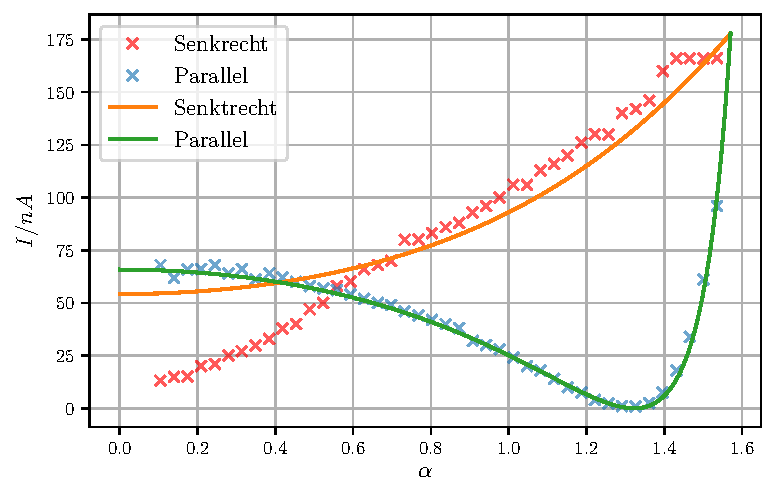
\includegraphics[]{build/plot1.pdf}
\end{figure}